As shown in Figure ~\ref{fig:linearity_test_plots}, all four dyes exhibited a linear correlation between concentration and signal intensity. To allow a consistent comparison between the fluorescent dyes, a signal intensity value of 0.2 was used, within the linear range for all dyes, to determine the
corresponding concentrations in the liquid combination phantom experiments. The concentration required to reach this signal varied by dye: AF700 required the lowest concentration ($21.30 nM$), followed by AF750 ($46.28 nM$), IR680 ($92.68 nM$), and IR800 ($282.00 nM$).

In the combination experiments, fluorescence intensity measurements were collected for individual dyes and their binary mixtures using ImageJ. These analyzed results are summarized in Figures ~\ref{fig:combo_700} and ~\ref{fig:combo_800}.

\begin{figure}[H]
    \centering
    \begin{minipage}{.94\linewidth}
        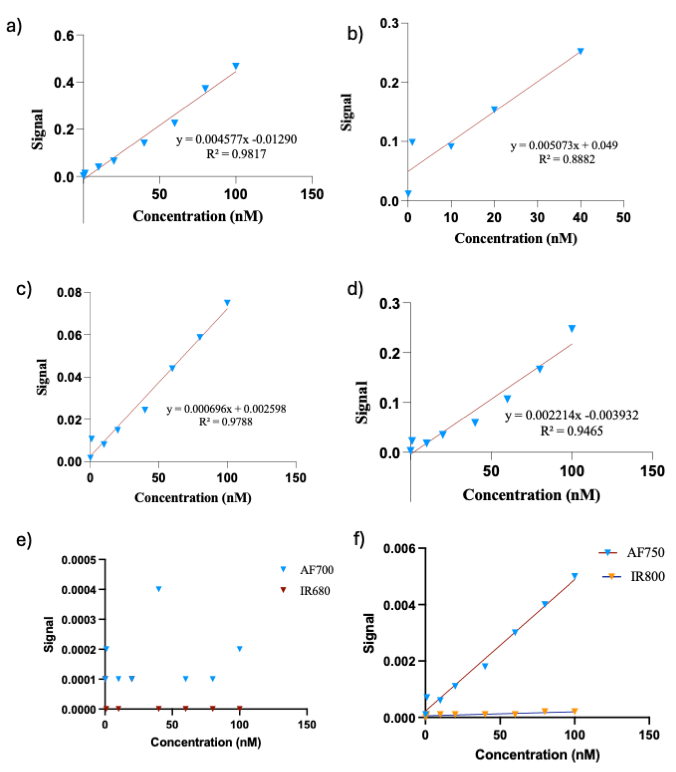
\includegraphics[width=\linewidth]{Thesis Template - LaTeX/figures/linearty_tests_plots.png}
        \begin{minipage}{0pt}
            \phantomsubcaption\label{fig:linearity_test_plots_a}
            \phantomsubcaption\label{fig:linearity_test_plots_b}
            \phantomsubcaption\label{fig:linearity_test_plots_c}
            \phantomsubcaption\label{fig:linearity_test_plots_d}
            \phantomsubcaption\label{fig:linearity_test_plots_e}
            \phantomsubcaption\label{fig:linearity_test_plots_f}
        \end{minipage}
        \captionsetup{justification=raggedright, singlelinecheck=false}
        \caption[Linearity test results]{
            \textbf{Linearity of signal intensity as a function of dye concentration in the 700 nm and 800 nm detection channels.}
            (a-d) Calibration curves demonstrate linear relationships between dye concentration and signal intensity for each 
            fluorophore in its primary detection channel: (a) IR680 and (b) AF700 in the 700 nm channel; (c) AF750 and (d) IR800 in 
            the 800 nm channel. (e-f) Signal contribution from dyes in their non-primary detection channels (i.e., bleed-through): 
            (e) IR680 and AF700 in the 800 nm channel; (f) AF750 and IR800 in the 700 nm channel.  
            }
        \label{fig:linearity_test_plots}
    \end{minipage}
\end{figure}

\begin{figure}[H]
    \centering
    \begin{minipage}{\linewidth}
        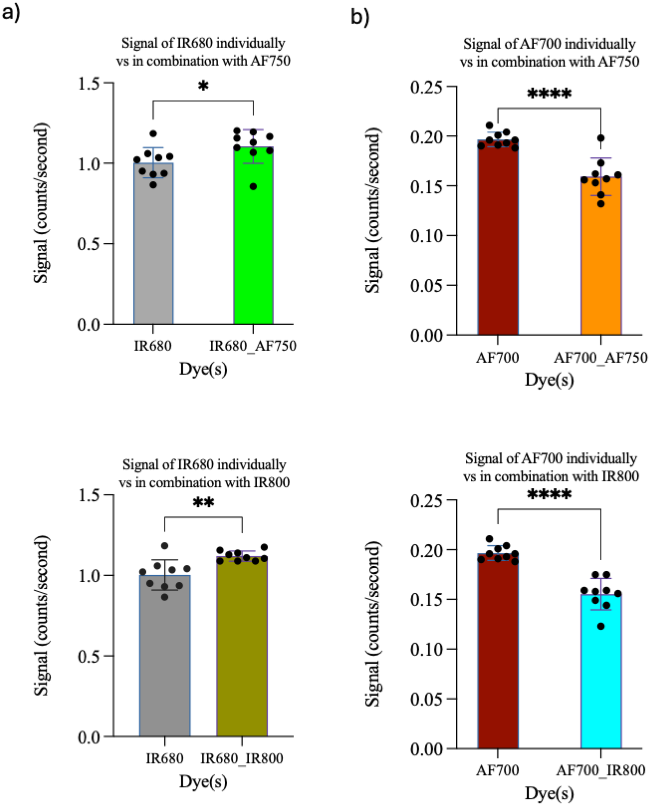
\includegraphics[width=\linewidth]{figures/combo_700nm.png}
        \captionsetup{justification=raggedright, singlelinecheck=false}
        \caption[Combination experiments results in  700nm channel]{
            \textbf{Fluorescence signal intensity comparisons in the 700 nm channel for individual dyes and binary combinations.} 
            (a) Signal intensity of IR680 alone vs. in combination with AF750 (top) and IR800 (bottom). (b) Signal intensity of AF700 
            alone vs. in combination with AF750 (top) and IR800 (bottom). Compared to AF700, IR680 showed minimal signal change when 
            combined with AF750 or IR800, indicating lower spectral cross-talk.
        }
        \label{fig:combo_700}
    \end{minipage}
\end{figure}

\begin{figure}[H]
    \centering
    \begin{minipage}{\linewidth}
        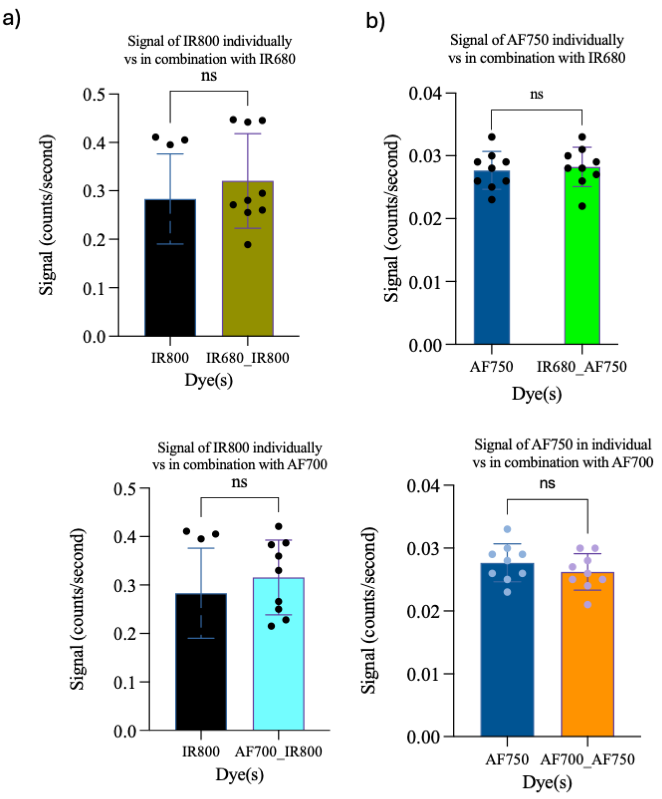
\includegraphics[width=\linewidth]{figures/combo_800.png}
        \captionsetup{justification=raggedright, singlelinecheck=false}
        \caption[Combination experiments results in 800nm channel]{
            \textbf{Fluorescence signal intensity comparisons in the 800 nm channel for individual dyes and binary combinations.} 
            (a) Signal intensity of AF750 alone vs. in combination with IR680 (top) and AF700 (bottom). (b) Signal intensity of 
            IR800 alone vs. in combination with IR680 (top) and AF700 (bottom). No significant changes in signal were observed, 
            indicating minimal spectral interference in the 800 nm channel.
        }
        \label{fig:combo_800}
    \end{minipage}
\end{figure}